\documentclass[]{article}

\usepackage{tikz}
\usepackage{amsmath}
\usepackage{amsfonts}
\usepackage{amssymb}
\usepackage{tkz-base}
\usepackage{tkz-euclide}
\usepackage{tikz-3dplot}
\usepackage{xcolor}
\usepackage{pgfplots}
\usepackage{graphicx}
\usepackage{url}
\usepackage{mathptmx}
\usepackage[american,siunitx]{circuitikz}
\usepackage{pgfplots}
\usepackage{cancel}
\usepackage{tabularray}
\usepgflibrary{patterns}
\usepackage{caption}
\usepackage{subcaption}

% Required packagef
\usetikzlibrary{positioning}
\usetikzlibrary{svg.path}
\usetikzlibrary{arrows}
\usetikzlibrary{shapes.geometric,calc}
\usetikzlibrary{calc,arrows.meta,backgrounds}
\usetikzlibrary{shapes, positioning, patterns, decorations, decorations.markings}
\usetikzlibrary{decorations.pathreplacing}
\usetikzlibrary { decorations.pathmorphing, decorations.shapes }
\usetikzlibrary{perspective}
\usetikzlibrary{3d}

\newcommand{\mymotor}[2] % #1 = name , #2 = rotation angle
{\draw[thick,rotate=#2] (#1) circle (10pt)
    node[]{$\mathsf M$} 
    ++(-12pt,3pt)--++(0,-6pt) --++(2.5pt,0) ++(-2.8pt,6pt)-- ++(2.5pt,0pt);
    \draw[thick,rotate=#2] (#1) ++(12pt,3pt)--++(0,-6pt) --++(-2.5pt,0) ++(2.8pt,6pt)-- ++(-2.5pt,0pt);
}

\newdimen\XCoord
\newdimen\YCoord
\newcommand*{\ExtractCoordinate}[1]{\path (#1); \pgfgetlastxy{\XCoord}{\YCoord};}%

\newcommand{\gear}[3]{%
  \def\modu{#1}
  \def\Zb{#2}
  \def\AngleA{#3}

  \pgfmathsetmacro{\Rpr}{\Zb*\modu/2}
  \pgfmathsetmacro{\Rb}{\Rpr*cos(\AngleA)}
  \pgfmathsetmacro{\Rt}{\Rpr+\modu}
  \pgfmathsetmacro{\Rp}{\Rpr-1.25*\modu}
  \pgfmathsetmacro{\AngleT}{pi/180*acos(\Rb/\Rt)}
  \pgfmathsetmacro{\AnglePr}{pi/180*acos(\Rb/\Rpr)}
  \pgfmathsetmacro{\demiAngle}{180/\Zb}
  \pgfmathsetmacro{\Angledecal}{(\demiAngle-2*\AnglePr)/2}

  \foreach \zz in{1,2,...,\Zb}{
    \draw
    ({(\zz))/\Zb*360-\Angledecal}:\Rb)
    -- (\zz/\Zb*360-\Angledecal:\Rp)
    to[bend right=\demiAngle]
    (\zz/\Zb*360+\Angledecal:\Rp)
    --
    plot[domain=-0:\AngleT,smooth,variable=\t]
    ({{180/pi*(-\t+tan(180/pi*\t)) +\zz/\Zb*360+\Angledecal}:\Rb/cos(180/pi*\t)})
    % 
    to[bend right=\demiAngle]
    ({{180/pi*(\AngleT+tan(180/pi*-\AngleT)) +(\zz+1)/\Zb*360-\Angledecal}:
      \Rb/cos(180/pi*-\AngleT)})
    % 
    plot[domain=-\AngleT:-0,smooth,variable=\t]
    ({{180/pi*(-\t+tan(180/pi*\t)) +(\zz+1)/\Zb*360-\Angledecal}:\Rb/cos(180/pi*\t)});
  }
}

\usetikzlibrary {perspective} 
\newcommand\simplecuboid[3]{
	
	 \filldraw[fill=gray]  (tpp cs:x=0,y=0,z=0)
	    -- (tpp cs:x=0,y=#2,z=0)
	    -- (tpp cs:x=#1,y=#2,z=0)
	    -- (tpp cs:x=#1,y=0,z=0) -- cycle;
	\draw[densely dashed] (#1, 0, 0) -- (#1, 0, #3);
  	 \filldraw[fill=gray!50!white] (tpp cs:x=0,y=#2,z=0)
	    -- (tpp cs:x=0,y=#2,z=#3)
	    -- (tpp cs:x=#1,y=#2,z=#3)
	    -- (tpp cs:x=#1,y=#2,z=0) -- cycle;
	 \filldraw[fill=gray!80!white] (tpp cs:x=0,y=0,z=0)
	    -- (tpp cs:x=0,y=0,z=#3)
	    -- (tpp cs:x=0,y=#2,z=#3)
	    -- (tpp cs:x=0,y=#2,z=0) -- cycle;
	\draw[|<->|] ($(#1, #2+0.2, 0)$) -- ($(#1, #2+0.2, #3)$) node[midway, above] {$l$};
%	\draw[|<->|] ($(#1+0.5, 0, 0)$) -- ($(#1+0.5, #2, 0)$) node[midway, left] {$m_{o}$};
%	\draw[|<->|] ($(#1, 0, -0.2)$) -- ($(0, 0, -0.2)$) node[left] {$m_{o}$};
 }

\newcommand\simplecuboidtwo[3]{
	
	 \filldraw[fill=gray]  (tpp cs:x=0,y=0,z=#3)
	    -- (tpp cs:x=0,y=#2,z=#3)
	    -- (tpp cs:x=#1,y=#2,z=#3)
	    -- (tpp cs:x=#1,y=0,z=#3) -- cycle;
	\draw[densely dashed] (#1, 0, 0) -- (#1, 0, #3);
  	 \filldraw[fill=gray!50!white] (tpp cs:x=0,y=#2,z=0)
	    -- (tpp cs:x=0,y=#2,z=#3)
	    -- (tpp cs:x=#1,y=#2,z=#3)
	    -- (tpp cs:x=#1,y=#2,z=0) -- cycle;
	 \filldraw[fill=gray!80!white] (tpp cs:x=0,y=0,z=0)
	    -- (tpp cs:x=0,y=0,z=#3)
	    -- (tpp cs:x=0,y=#2,z=#3)
	    -- (tpp cs:x=0,y=#2,z=0) -- cycle;
	\draw[|<->|] ($(#1, #2+0.2, 0)$) -- ($(#1, #2+0.2, #3)$) node[midway, above] {50 cm};
%	\draw[|<->|] ($(#1+0.5, 0, 0)$) -- ($(#1+0.5, #2, 0)$) node[midway, left] {$m_{o}$};
%	\draw[|<->|] ($(#1, 0, -0.2)$) -- ($(0, 0, -0.2)$) node[left] {$m_{o}$};
 }

\newcommand{\simpleaxes}[3]{%
  \draw[->] (-0.5,0,0) -- (#1,0,0) node[pos=1.1]{x};
  \draw[->] (0,-0.5,0) -- (0,#2,0) node[pos=1.1]{y};
  \draw[->] (0,0,-0.5) -- (0,0,#3) node[pos=1.1]{z};}

\newcommand{\tikzmark}[1]{\tikz[overlay,remember picture] \node (#1) {};}
\newcommand{\DrawBox}[2]{%
  \begin{tikzpicture}[overlay,remember picture]
    \draw[->,shorten >=5pt,shorten <=5pt,out=0,in=180,distance=0.5cm,#1] (MarkA.east) to ($(MarkA.east)+(1.5cm, 0.25cm)$) node [right]{stiffness};
    \draw[->,shorten >=5pt,shorten <=5pt,out=0,in=180,distance=0.3cm,#2] (MarkB.east) to ($(MarkB.east)+(1.5cm, -0.25cm)$) node[right] {effective mass or inertia};
  \end{tikzpicture}
}

%opening
\title{Modelling of Stiffness}
\author{Craig Carignan \& Glen Henshaw}

\begin{document}
\maketitle

\section{Intro}
We're going to talk about how to model the flexibility of a joint. Real mechanisms are never infinitely stiff, although with many robotic mechanisms the stiffness is high enough that we can mostly ignore it, or at least design suitable control laws such that we don't excite flex modes. In some cases, however, that isn't possible. Very long robot arms, such as the SRMS and SSRMS, have nontrivial flex dynamics that need to be modeled and managed, either via appropriate control laws or via operational procedures. Also, there is emerging research in soft robotics where the flexibility of a manipulator is in fact one of its defining features.

That being said, this isn't going to be a lecture so much as it is a summary of the types of flexible structures and mechanisms you might encounter in the wild and accepted equations for modeling them. We aren't going to derive or even really motivate these models; the modeling of deformable structures is at least an entire graduate--level class.

One introductory note: if you have two or more structural elements in combination, you can find the flexibility of the assembly as follows.

\begin{tblr}{
  colspec = {Q[m]Q[m]Q[m]Q[m]},
  stretch = 0,
  rowsep = 6pt,
  hlines = {red5, 0pt},
  vlines = {red5, 0pt},
}
	&&&\\
	Type & Diagram & Example & Equation \\
	&&&\\
	Parallel & 
         \parbox{4cm}{
         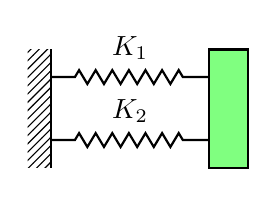
\begin{tikzpicture}[every node/.style={outer sep=0pt},thick,
		mass/.style={draw,thick},
		spring/.style={thick,decorate,decoration={zigzag,pre length=0.3cm,post
		length=0.3cm,segment length=6}},
		ground/.style={fill,pattern=north east lines,draw=none,minimum
		width=0.75cm},
		]
		\node[mass,minimum width=0.5cm,minimum height=1.5cm,fill=green!50] (m1) {};
               \node[left=2cm of m1,ground,minimum width=3mm,minimum height=1.5cm] (g1){};
              \draw (g1.north east) -- (g1.south east);
            
              \draw[spring] ([yshift=4mm]g1.east) coordinate(aux)
               -- (m1.west|-aux) node[midway,above=1mm]{$K_{1}$};
            
              \draw[spring] ([yshift=-4mm]g1.east) coordinate(aux)
               -- (m1.west|-aux) node[midway,above=1mm]{$K_{2}$};
            
        \end{tikzpicture}}
	& 
	\parbox{2.5cm}{
	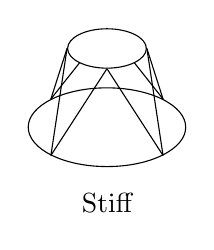
\begin{tikzpicture}
	\tikzset{
  		shape example 1/.style= {color = black,draw}
		}
		 \path 	(0,0) node [name=lower, shape=ellipse, shape example 1, minimum width=2cm, minimum height=1cm] {}
		 		(0,1) node [name=upper, shape=ellipse, minimum width=1cm, minimum height=0.5cm] {};

		\draw (lower.south west) -- (upper.south);
		\draw (lower.south east) -- (upper.south);
		\draw (lower.south east) -- (upper.east);
		\draw (lower.north east) -- (upper.east);
		\draw (lower.north east) -- (upper.north);
		\draw (lower.north west) -- (upper.north);
		\draw (lower.south west) -- (upper.west);
		\draw (lower.north west) -- (upper.west);
		\draw (lower.south) node [below=6pt] {Stiff};
		\path (0,1) node [shape=ellipse, shape example 1, fill=white, minimum width=1cm, minimum height=0.5cm] {};

	\end{tikzpicture}}
	& $K_{\text{par}} = K_{1}+K_{2}$ \\
	Series &
	\parbox{4cm}{
         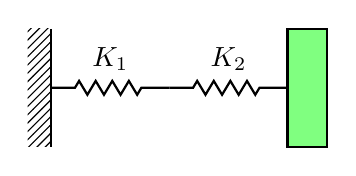
\begin{tikzpicture}[every node/.style={outer sep=0pt},thick,
		mass/.style={draw,thick},
		spring/.style={thick,decorate,decoration={zigzag,pre length=0.3cm,post
		length=0.3cm,segment length=6}},
		ground/.style={fill,pattern=north east lines,draw=none,minimum
		width=0.75cm},
		]
		\node[mass,minimum width=0.5cm,minimum height=1.5cm,fill=green!50] (m1) {};
		\node[left=3cm of m1,ground,minimum width=3mm,minimum height=1.5cm] (g1){};
		\draw (g1.north east) -- (g1.south east);
            
            	\coordinate(C) at ($ (g1.east)!1.5cm!(m1.west) $);

		\draw[spring] (g1.east)  -- (C) node[midway,above=1mm]{$K_{1}$};
            	\draw[spring] (C)  -- (m1.west) node[midway,above=1mm]{$K_{2}$};            
        \end{tikzpicture}}
 & 
 	\parbox{2.5cm} {
	
\begin{tikzpicture}
		\draw [line cap=round, line width=1pt, double distance=6pt] (0,0) -- (1, -0.5);
		\draw [line cap=round, line width=1pt, double distance=6pt] (1, -0.5) -- (2, 0);
		\draw (1, -0.5) circle (1pt);
		\draw (1, -0.5) node [below=8pt] {Not stiff};
	\end{tikzpicture}}
 & $\frac{1}{K_{\text{ser}}} = \frac{1}{K_{1}}+\frac{1}{K_{2}}$ \\
\end{tblr}

\section{Flexible Elements}
    \begin{tblr}{lll}
%      colspec = {lll},
%      stretch = 0,
%      rowsep = 6pt,
%      hlines = {black, 0pt},
%      vlines = {black, 0pt},
%    }
   	Shaft &
	\parbox{8cm}{\centering
	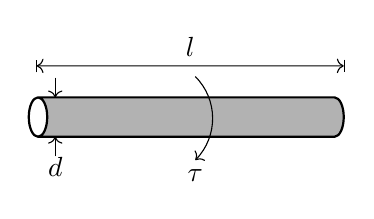
\begin{tikzpicture}
		\draw (0,0) node[cylinder,draw=black,thick,minimum height=4cm,minimum width=0.5cm,rotate=180,cylinder uses custom fill, cylinder body fill=black!30,cylinder, name=shaft]{};
		\draw [->] ($(shaft.south)+(0cm,0.25cm)$) arc (45:-45:0.75) node [below]{$\tau$};
		\draw [|<->|] ($(shaft.west)+(0cm,0.65cm)$) -- ($(shaft.east)+(0.1cm,0.65cm)$) node[midway,above] {$l$};
		\draw [->] ($(shaft.east)+(0.35cm, 0.5cm)$) -- ($(shaft.east)+(0.35cm, 0.25cm)$);
		\draw [->] ($(shaft.east)+(0.35cm, -0.5cm)$) -- ($(shaft.east)+(0.35cm, -0.25cm)$) node [below=4pt]{$d$};
	\end{tikzpicture}}
	& \parbox{5cm}{$K = \frac{G\pi d^{4}}{32l}$\\where $G$ is the ``shear modulus''\\(steel = $7.5\times10^{10}$ N/m$^{2}$)}
	\\
    	Gear &
	\parbox{7cm}{\centering
	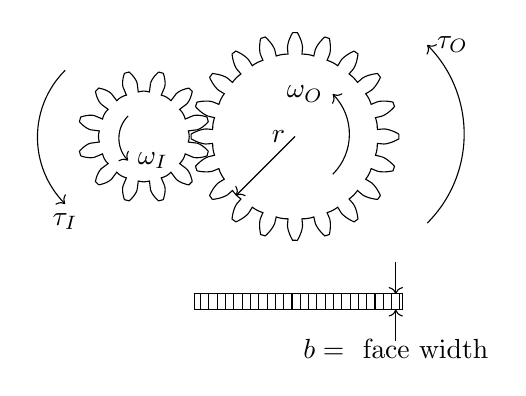
\begin{tikzpicture}[scale=0.04]
		\gear{3}{12}{20}
		\begin{scope}[xshift=48cm,rotate=180/20]
		\gear{3}{20}{20}
		\end{scope}
		\draw [->] (90cm,-27.5cm) arc (-45:45:40cm) node [above,right] {$\tau_{O}$};
		\draw [->] (-25cm,21cm) arc (135:225:30cm) node [below] {$\tau_{I}$};
		\draw [->] (60cm,-12cm) arc (-45:45:18cm) node [left] {$\omega_{O}$};
		\draw [->] (-5cm,6.5cm) arc (135:225:10cm) node [right] {$\omega_{I}$};
		\draw [->] (48cm,0cm) node [left]{$r$} -- ++ (canvas polar cs:angle=225,radius=26.5cm);
		\draw[pattern=vertical lines] (16cm, -50cm) rectangle (82cm, -55cm);
		\draw[->] (80, -40) -- (80, -50);
		\draw[->] (80, -65) -- (80, -55) node [below=0.25cm] {$b =\ $ face width};
		%\draw (0cm,0cm) -- (30:1cm) -- (60:1cm) -- (90:1cm) -- (120:1cm) -- (150:1cm) -- (180:1cm);
	\end{tikzpicture}} &
	\parbox{2cm}{
		\begin{eqnarray}
			r & = & \text{radius of output gear} \nonumber \\
			\eta & = & \text{gear ratio} \nonumber\\
			\omega_{O} & = & \frac{\omega_{I}}{\eta} \nonumber\\
			\tau_{O} & = & \tau_{I}\eta\ \nonumber \\ %\text{(assume $\eta_{\text{gear}} = 1$)} \nonumber \\
			K & = & C_{g}br^{2}\ \text{(locked input gear)} \nonumber \\
			C_{g} & = & 1.34\times 10^{10}\ \text{N/m}^{2}\ \text{(steel)} \nonumber
		\end{eqnarray}}
	\\
     	&
	\parbox{7cm}{\centering
	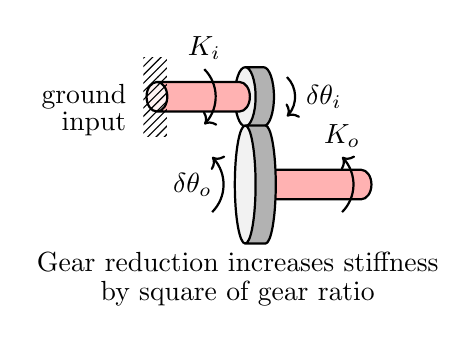
\begin{tikzpicture}[every node/.style={outer sep=0pt},thick,
		mass/.style={draw,thick},
		spring/.style={thick,decorate,decoration={zigzag,pre length=0.3cm,post
		length=0.3cm,segment length=6}},
		ground/.style={fill,pattern=north east lines,draw=none,minimum
		width=0.75cm}
		]
			
		\coordinate(A) at (-0.5,0);
		\coordinate(B) at (5cm, 0cm);
		\coordinate(C) at ($ (A)!1.125cm!(B) $);
		\coordinate(E) at ($ (C)!0.7cm!(B) $);
		\coordinate(F) at ($(E)!1.115cm!-90:(B) $);
		\coordinate(G) at ($(F)+(3.75cm,0cm)$);
		\coordinate(H) at ($(F)!0.75cm!(G)$);
		\coordinate(I) at ($(H)!0.95cm!(G)$);
		\coordinate(J) at ($(I)!1cm!(G)$);
		
		\draw (E) node[cylinder,draw=black,thick,aspect=1.5,minimum height=0.25cm,minimum width=1cm,rotate=180,cylinder uses custom fill, cylinder body fill=black!30,cylinder end fill=black!5,scale=0.75]{};
		\draw (C) node[cylinder,draw=black,thick,aspect=1.5,minimum height=1.75cm,minimum width=0.5cm,rotate=180,cylinder uses custom fill, cylinder body fill=red!30,cylinder end fill=red!5,scale=0.75]{};
		\path (-0.05,0) node[ground,minimum width=3mm,minimum height=1cm] (g1){} node[left=0.25cm]{ground} ++(0, -0.35) node[left=0.25cm]{input};
		\draw (H) node[cylinder,draw=black,thick,aspect=1.5,minimum height=2cm,minimum width=0.5cm,rotate=180,cylinder uses custom fill, cylinder body fill=red!30,cylinder end fill=red!5,scale=0.75]{};
		\draw (F) node[cylinder,draw=black,thick,aspect=1.5,minimum height=0.25cm,minimum width=2cm,rotate=180,cylinder uses custom fill, cylinder body fill=black!30,cylinder end fill=black!5,scale=0.75]{};
		\draw[->] ($(E.north)+(-0.75cm, 0.35cm)$) node[above] {$K_{i}$ }to[out=-45,in=45] ($(E.south)+(-0.75cm, -0.35cm)$);
		\draw[->] ($(C.west)+(1cm, 0.25cm)$) to[out=-45,in=45]  ($(C.west)+(1cm, -0.25cm)$) node[midway, right=1.75cm] {$\delta\theta_{i}$};
		\draw[->] ($(H.west)+(0.25cm, -0.35cm)$) to[in=-45, out=45]  ($(H.west)+(0.25cm, 0.35cm)$) node[above] {$K_{o}$};
		\draw[->] ($(F)+(-0.65, -0.35)$) to[in=-45, out=45] ($(F)+(-0.65, 0.35)$);
		\path ($(F)+(-0.9, 0)$) node {$\delta\theta_{o}$};
		\path (1cm, -2.1cm) node {Gear reduction increases stiffness};
		\path (1cm, -2.5cm) node {by square of gear ratio};
	\end{tikzpicture}} &
	\parbox{2cm}{
		\begin{eqnarray}
			\tau_{i} & = & K_{i}\delta \theta_{i} \nonumber \\
			\tau_{o} & = & K_{o}\delta \theta_{o} \nonumber\\
			K_{o} & = & \frac{\tau_{o}}{\delta\theta_{o}} = \frac{\eta\tau_{i}}{\delta\theta_{i}/\eta} \nonumber \\
			& = & \frac{\eta K_{i}\cancelto{}{\delta\theta_{i}}}{\cancelto{}{\delta\theta_{i}}/\eta} = \eta^{2}K_{i} \nonumber
		\end{eqnarray}}
	\\
   	Belt &
		\parbox{8cm}{\centering
        		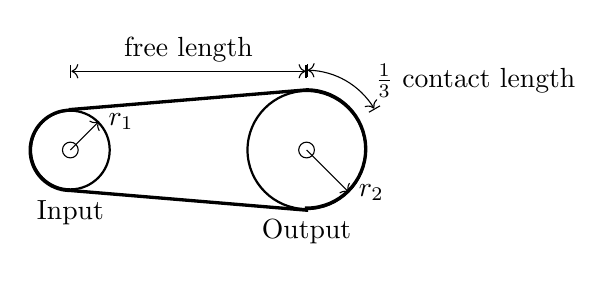
\begin{tikzpicture}
			\draw[thick] (3cm,0cm) node[circle, draw=black, minimum size=1.5cm, name=big] {};
			\draw[thick] (0cm,0cm) node[circle, draw=black, minimum size=1cm, name=small] {};
			\draw[very thick] (small.north) -- (big.north) arc (90:-90:0.751cm) -- (big.south) -- (small.south) arc (270:90:0.51cm) -- cycle;
			\draw (3cm,0cm) circle[radius=0.1cm];
			\draw (0cm,0cm) circle[radius=0.1cm];
			\draw (big.south) node[below] {Output};
			\draw (small.south) node[below] {Input};
			\draw[->] (big.base) -- (big.south east) node [right] {$r_{2}$};
			\draw[->] (small.base) -- (small.north east) node [right] {$r_{1}$};
			\draw[|<->|] (0cm, 1cm) -- (3cm, 1cm) node[midway,above] {free length};
			\draw[|<->|] (big.north)++(0cm, 0.25cm) arc (90:30:1cm) node[midway,right=0.25cm] {$\frac{1}{3}\ $contact length};
       	 	\end{tikzpicture}} &
		\parbox{2cm}{
			\begin{eqnarray}
				K & = & \frac{AE}{l} \nonumber \\
				A & = & \text{cross sectional area of belt} \nonumber \\
				E & = & \text{modulus of elasticity} \nonumber \\
				l & = & \text{free length}+\frac{1}{3}\ \text{contact length} \nonumber
			\end{eqnarray}}
	\\
    	Link&
		\parbox{8cm}{\centering
		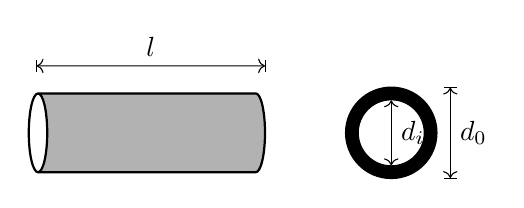
\begin{tikzpicture}
			\draw (0,0) node[cylinder,draw=black,thick,minimum height=3cm,minimum width=1cm,rotate=180,cylinder uses custom fill, cylinder body fill=black!30,cylinder, name=link]{};
			\draw [|<->|] ($(link.west)+(0cm,0.85cm)$) -- ($(link.east)+(0.1cm,0.85cm)$) node[midway,above] {$l$};
			\draw[line width=5pt] (3cm, 0cm) node[circle,draw=black,name=circ, minimum size=1cm] {};
			\draw[<->] ($(3cm, -0.5cm+2.5pt)$) -- ($(3cm, 0.5cm-2.5pt)$) node[midway, right=0cm]{$d_{i}$};
			\draw[|<->|] ($(3.75cm, -0.5cm-2.5pt)$) -- ($(3.75cm, 0.5cm+2.5pt)$) node[midway, right]{$d_{0}$};
		\end{tikzpicture}} &
		\parbox{2cm}{
			\begin{eqnarray}
				K & = & \frac{3\pi E(d_{o}^{4}-d_{i}^{4})}{64l^{3}} \nonumber \\
				E & = & 2\times10^{11}\ \text{N/m}^{2}\ \text{(steel)} \nonumber \\
				&=& \frac{2}{3}\times 10^{11}\ \text{N/m}^{2}\ \text{(aluminum)} \nonumber
			\end{eqnarray}
		}
	\\
	&
	\parbox{8cm}{\centering
	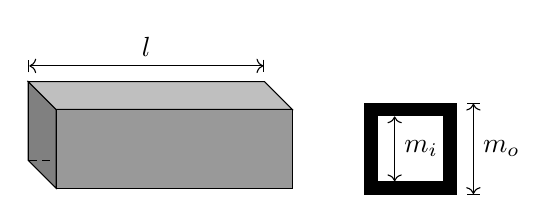
\begin{tikzpicture}[z={(0:10mm)},x={(135:5mm)}]
		\simplecuboid{1}{1}{3}
		%\simpleaxes{1}{1}{1}
		\draw[line width=5pt] (4cm,0cm) rectangle (5cm,1cm);
		\draw[<->] ($(4.3cm, 0cm+2.5pt)$) -- ($(4.3cm, 1cm-2.5pt)$) node[midway, right]{$m_{i}$};
		\draw[|<->|] ($(5.3cm, 0cm-2.5pt)$) -- ($(5.3cm, 1cm+2.5pt)$) node[midway, right]{$m_{o}$};
	\end{tikzpicture}} &
	\parbox{2cm}{\begin{flushleft}
	\begin{eqnarray}
		K & = & \frac{E(w_{o}^{4} - w_{i}^{4})}{4l^{3}} \nonumber
	\end{eqnarray}
	\end{flushleft}
	}
	\\
    \end{tblr}

\section{Example: Gear Stiffness} %

What is the output stiffness of the drive system below?

\begin{figure}[h!]
	\centering
	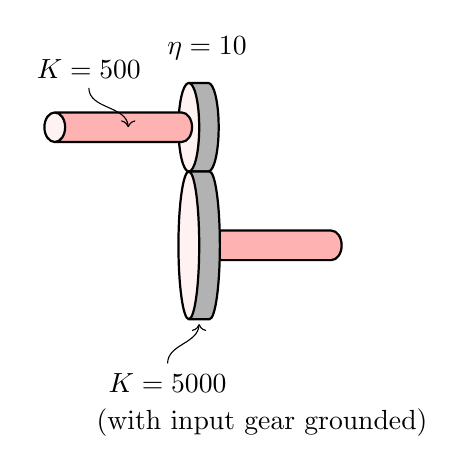
\begin{tikzpicture}
		\coordinate(A) at (0cm,0cm);
		\coordinate(B) at (5cm, 0cm);
		\coordinate(C) at ($ (A)!1.25cm!(B) $);
		\coordinate(D) at ($ (A)!-0.95cm!(B) $);
		\coordinate(E) at ($ (C)!1cm!(B) $);
		\coordinate(F) at ($(E)!1.5cm!-90:(B) $);
		\coordinate(G) at ($(F)+(3.75cm,0cm)$);
		\coordinate(H) at ($(F)!0.9cm!(G)$);
		\coordinate(I) at ($(H)!0.95cm!(G)$);
		\coordinate(J) at ($(I)!1cm!(G)$);
		
		\draw (E) node[cylinder,draw=black,thick,aspect=1.5,minimum height=0.5cm,minimum width=1.5cm,rotate=180,cylinder uses custom fill, cylinder body fill=black!30,cylinder end fill=red!5,scale=0.75]{};
		\draw (C) node[cylinder,draw=black,thick,aspect=1.5,minimum height=2.5cm,minimum width=0.5cm,rotate=180,cylinder uses custom fill, cylinder body fill=red!30,cylinder end fill=red!5,scale=0.75]{};
		\draw (H) node[cylinder,draw=black,thick,aspect=1.5,minimum height=2.5cm,minimum width=0.5cm,rotate=180,cylinder uses custom fill, cylinder body fill=red!30,cylinder end fill=red!5,scale=0.75]{};
		\draw (F) node[cylinder,draw=black,thick,aspect=1.5,minimum height=0.5cm,minimum width=2.5cm,rotate=180,cylinder uses custom fill, cylinder body fill=black!30,cylinder end fill=red!5,scale=0.75]{};
		\draw [<-] (C) to[out=90, in=-90] ($(C)+(-0.5cm, 0.5cm)$) node[above] {$K=500$};
		\draw ($(E) + (0cm, 1cm)$) node{$\eta=10$};
		\draw [<-] ($(F)-(0.1cm, 1cm)$) to[in=90, out=-90] ($(F)-(0.5cm, 1.5cm)$) node[below] {$K=5000$};
		\draw ($(F)-(-0.7cm, 2.25cm)$) node {(with input gear grounded)};
	\end{tikzpicture}
\end{figure}

\begin{eqnarray}
	\frac{1}{K_{sys}} & = & \frac{1}{K_{gear}} + \frac{1}{K_{shaft}} \nonumber \\
	& = & \underbrace{\frac{1}{500}}_{\text{at output}} + \underbrace{\frac{1}{(10)^{2}(500)}}_{50000} \nonumber \\
	K_{sys} & = & 4545\ \text{ N-m/rad} \nonumber
\end{eqnarray}
\section{Example}
\begin{figure}[h!]
	\centering
	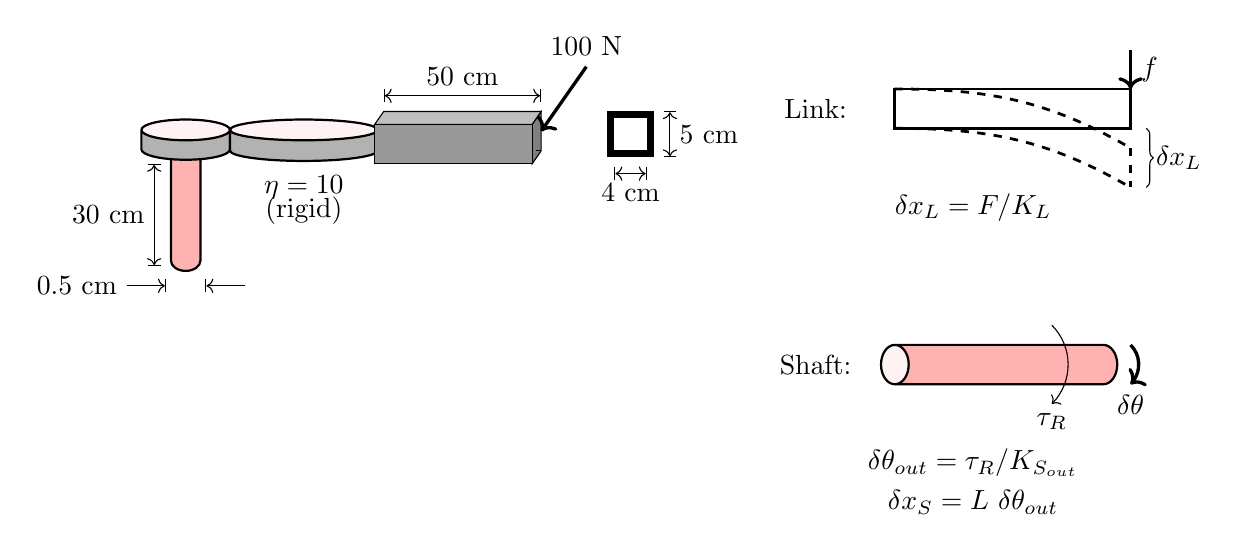
\begin{tikzpicture}
		\coordinate(A) at (0cm,0cm);
		\coordinate(B) at (0cm, 5cm);
		\coordinate(C) at (A);
		\coordinate(D) at ($ (A)!-0.95cm!(B) $);
		\coordinate(E) at ($ (C)!0.75cm!(B) $);
		\coordinate(F) at ($(E)!-1.5cm!90:(B) $);
		\coordinate(G) at ($(F)+(0cm, 3.75cm)$);
		\coordinate(H) at ($(F)!0.5cm!(G)$);
		\coordinate(I) at ($(H)!0.95cm!(G)$);
		\coordinate(J) at ($(I)!1cm!(G)$);

		\draw (C) node[cylinder,draw=black,thick,aspect=1.5,minimum height=2.5cm,minimum width=0.5cm,rotate=90,cylinder uses custom fill, cylinder body fill=red!30,cylinder end fill=red!5,scale=0.75]{};
		\draw (E) node[cylinder,draw=black,thick,aspect=1.5,minimum height=0.5cm,minimum width=1.5cm,rotate=90,cylinder uses custom fill, cylinder body fill=black!30,cylinder end fill=red!5,scale=0.75]{};
		\draw (F) node[cylinder,draw=black,thick,aspect=1.5,minimum height=0.5cm,minimum width=2.5cm,rotate=90,cylinder uses custom fill, cylinder body fill=black!30,cylinder end fill=red!5,scale=0.75]{};
		\draw[|<->|] ($(C)-(0.4cm, 0.75cm)$) -- ($(E)-(0.4cm, 0.2cm)$) node[midway, left] {30 cm};
		\draw ($(F)-(0,0.5cm)$) node {$\eta=10$};
		\draw ($(F)-(0,0.8cm)$) node {(rigid)};
		\draw [->|] (-0.75, -1cm)node[left] {0.5 cm} -- (-0.25cm, -1cm);
		\draw [->|] (0.75, -1cm)-- (0.25cm, -1cm);
		%\simpleaxes{1}{1}{1};
		\begin{scope}[xshift=2.4cm, yshift=0.55cm]
			\begin{scope}[z={(0:10mm)}, x={(55:4mm)}]
				\simplecuboidtwo{0.5}{0.5}{2}
				\draw [very thick,<-] (0.5,0.25,2) -- (3,0.25,2) node[above] {100 N};
				\draw[line width=2.5pt] (3cm,0.125cm) rectangle (3.5cm,0.625cm);
				\draw[|<->|] ($(3.75cm, 0.125cm-1.25pt)$) -- ($(3.75cm, 0.625cm+1.25pt)$) node[midway, right]{5 cm};
				\draw[|<->|] ($(3cm+1.25pt, -0.125cm)$) -- ($(3.5cm-1.25pt, -0.125cm)$) node[midway, below]{4 cm};
			\end{scope}
		\end{scope}
		\begin{scope}[xshift=8cm,yshift=1cm]
			\draw[line width=1pt] (0,0.25) node {Link:} (1cm,0cm) rectangle (4cm,0.5cm);
			\draw[line width=1pt, dashed] (1cm, 0cm) to[out=0, in=150] (4cm, -0.75cm);
			\draw[line width=1pt, dashed] (1cm, 0.5cm) to[out=0, in=150] (4cm, -0.25cm);
			\draw[line width=1pt, dashed] (4cm, -0.25cm) -- (4cm, -0.75cm);
			\draw[->, very thick] (4cm, 1cm) -- node[midway,right]{$f$} (4cm, 0.5cm);
			\draw[decoration={brace},decorate] (4.2cm, 0cm) -- node[midway, right] {$\delta x_{L}$} (4.2cm, -0.75cm);
			\draw (2cm, -1cm) node{$\delta x_{L} = F/K_{L}$};
		\end{scope}
		\begin{scope}[xshift=8cm,yshift=-2cm]
			\draw[line width=1pt] (0,0) node {Shaft:} (2.5cm,0cm) node[cylinder,draw=black,thick,aspect=1.5,minimum height=3cm,minimum width=0.5cm,rotate=180,cylinder uses custom fill, cylinder body fill=red!30,cylinder end fill=red!5]{};
			\draw [->] (3, 0.5) to[out=-45,in=45] (3, -0.5) node[below] {$\tau_{R}$};
			\draw [->, very thick] (4, 0.25) to[out=-45,in=45] (4, -0.25) node[below] {$\delta \theta$};
			\draw (2cm, -1.25cm) node{$\delta \theta_{out} = \tau_{R}/K_{S_{out}}$};
			\draw (2cm, -1.75cm) node{$\delta x_{S} = L\ \delta\theta_{out}$};
		\end{scope}		
	\end{tikzpicture}
\end{figure}
\begin{eqnarray}
	K_{shaft} & = & \frac{G\pi d^{4}}{32 l} = \frac{(7.5\times16^{10})(\pi)(5\times 10^{-3})^{4}}{32(0.3)} = 15.3\ \text{N-m/rad} \rightarrow K_{S_{out}} = 15.3(10)^{2} = 1530\ \text{N/m}^{2} \nonumber \\
	K_{link} & = & \frac{E(w_{o}^{4}-w_{i}^{4})}{4l^{3}} = \frac{(2\times10^{11})(0.05^{4}-0.04^{4})}{4(0.5)^{3}} = 1.476\times 10^{-5}\ \text{N/m} \nonumber
\end{eqnarray}
Link: $\delta x_{L} = 100\ \text{N}/1.476\times10^{6}\ \text{N-m} = 6.78\times 10^{-5}\ \text{m}$

\noindent
Shaft: $\delta x_{S} = (0.50\ \text{m})(0.5\ \text{m} \times100\ \text{N})/1530\ \text{N/m}^{2} = 0.0163\ \text{m}$

\section{Estimating $\omega_{r}$}

\begin{figure}[h!]
	\centering
	\begin{equation}
		\omega_{n} = \sqrt{\frac{k\tikzmark{MarkA}}{m\tikzmark{MarkB}}} \DrawBox{black}{black} \nonumber
	\end{equation}
\end{figure}

\subsection{Example: Shaft}
\begin{figure}[h!]
	\centering
	\begin{minipage}{.5\textwidth}\centering
    	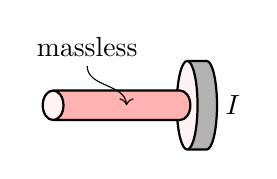
\begin{tikzpicture}
    		\coordinate(A) at (0cm,0cm);
    		\coordinate(B) at (5cm, 0cm);
    		\coordinate(C) at ($ (A)!1.25cm!(B) $);
    		\coordinate(D) at ($ (A)!-0.95cm!(B) $);
    		\coordinate(E) at ($ (C)!1cm!(B) $);
    		\coordinate(F) at ($(E)!1.5cm!-90:(B) $);
    		\coordinate(G) at ($(F)+(3.75cm,0cm)$);
    		\coordinate(H) at ($(F)!0.9cm!(G)$);
    		\coordinate(I) at ($(H)!0.95cm!(G)$);
    		\coordinate(J) at ($(I)!1cm!(G)$);
    		
    		\draw (E) node[cylinder,draw=black,thick,aspect=1.5,minimum height=0.5cm,minimum width=1.5cm,rotate=180,cylinder uses custom fill, cylinder body fill=black!30,cylinder end fill=red!5,scale=0.75]{};
    		\draw ($(E)+(0.35cm,0cm)$) node{$I$};
    		\draw (C) node[cylinder,draw=black,thick,aspect=1.5,minimum height=2.5cm,minimum width=0.5cm,rotate=180,cylinder uses custom fill, cylinder body fill=red!30,cylinder end fill=red!5,scale=0.75]{};
    		\draw [<-] (C) to[out=90, in=-90] ($(C)+(-0.5cm, 0.5cm)$) node[above] {massless};
    	\end{tikzpicture}
	\end{minipage}%
	\begin{minipage}{.5\textwidth}\centering
		\begin{eqnarray}
			k & = & 400\  \text{N-m/rad} \nonumber \\
			I & = & 1\ \text{kg-m}^{2} \nonumber \\
			\omega_{r} & = & \sqrt{\frac{400}{m}} = 20\ \text{rad/sec} = 3.2\ \text{Hz} \nonumber
		\end{eqnarray}
	\end{minipage}
\end{figure}

\noindent
\subsection{Lumped mass model}

\begin{figure}[h!]\centering
	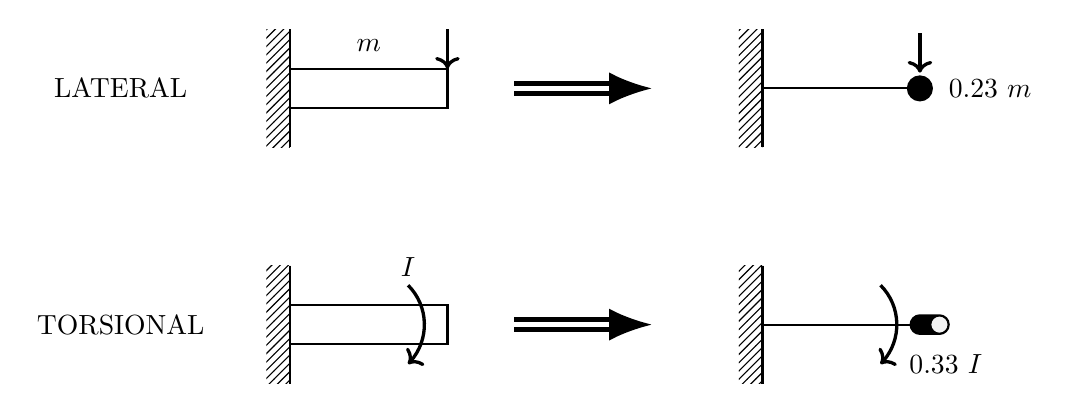
\begin{tikzpicture}[every node/.style={outer sep=0pt},thick,
		mass/.style={draw,thick},
		spring/.style={thick,decorate,decoration={zigzag,pre length=0.3cm,post
		length=0.3cm,segment length=6}},
		ground/.style={fill,pattern=north east lines,draw=none,minimum
		width=0.75cm},
		]
		\begin{scope}[xshift=-6cm,yshift=0cm]
			\path(0,0) node {LATERAL};
		\end{scope}
		\begin{scope}[xshift=-1cm,yshift=0cm]
			\path (-3,0) node[ground,minimum width=3mm,minimum height=1.5cm] (g1){};
			 \draw (g1.north east) -- (g1.south east);
			\draw ($(g1.east)+(0cm, -0.25cm)$) rectangle ($(g1.east)+(2cm, 0.25cm)$) node[midway, above=0.35cm]{$m$};
			\draw[<-, very thick] ($(g1.east)+(2cm, 0.25cm)$) -- ($(g1.east)+(2cm, 0.75cm)$);
		\end{scope}
		\begin{scope}[xshift=2cm,yshift=0cm]
			\draw[ultra thick, double distance=2pt, arrows = {-Latex[length=0pt 3 0]}] (-3cm,0cm) -- (-1.25cm,0cm);
		\end{scope}
		\begin{scope}[xshift=5cm,yshift=0cm]
			\path (-3,0) node[ground,minimum width=3mm,minimum height=1.5cm] (g1){};
			 \draw (g1.north east) -- (g1.south east);
			\draw ($(g1.east)+(0cm, 0cm)$) -- ($(g1.east)+(2cm, 0cm)$) node[circle, fill=black, minimum size=0.1cm] {} node[right=0.25cm]{$0.23\ m$};
			\draw[<-, very thick] ($(g1.east)+(2cm, 0.2cm)$) -- ($(g1.east)+(2cm, 0.7cm)$);		
		\end{scope}

		\begin{scope}[xshift=-6cm,yshift=-3cm]
			\path(0,0) node {TORSIONAL};
		\end{scope}		
		\begin{scope}[xshift=-1cm,yshift=-3cm]
			\path (-3,0) node[ground,minimum width=3mm,minimum height=1.5cm] (g1){};
			\draw (g1.north east) -- (g1.south east);
			\draw ($(g1.east)+(0cm, -0.25cm)$) rectangle ($(g1.east)+(2cm, 0.25cm)$);
			\draw[->, very thick] ($(g1.east)+(1.5cm, 0.5cm)$) node [above] {$I$} to[out=-45,in=45] ($(g1.east)+(1.5cm, -0.5cm)$) ;
			%\draw[<-, very thick] ($(g1.east)+(2cm, 0.25cm)$) -- ($(g1.east)+(2cm, 0.75cm)$);
		\end{scope}
		\begin{scope}[xshift=2cm,yshift=-3cm]
			\draw[ultra thick, double distance=2pt, arrows = {-Latex[length=0pt 3 0]}] (-3cm,0cm) -- (-1.25cm,0cm);
		\end{scope}
		\begin{scope}[xshift=5cm,yshift=-3cm]
			\path (-3,0) node[ground,minimum width=3mm,minimum height=1.5cm] (g1){};
			\draw (g1.north east) -- (g1.south east);
			\draw ($(g1.east)+(0cm, 0cm)$) -- ($(g1.east)+(2cm, 0cm)$) node[cylinder,draw=black,thick,cylinder uses custom fill, cylinder body fill=black,cylinder end fill=black!5, minimum size=0.1cm] {};
			\draw[->, very thick] ($(g1.east)+(1.5cm, 0.5cm)$) to[out=-45,in=45] ($(g1.east)+(1.5cm, -0.5cm)$) node [right=0.25cm] {$0.33\ I$};
		\end{scope}

	\end{tikzpicture}
\end{figure}
\subsection{Example: 9.9: Link}
\begin{eqnarray}
	m & = & 4.347\ \text{kg} \nonumber \\
	k & = & 3600\ \text{N/m} \nonumber
\end{eqnarray}
What is $\omega_{r}$?

\noindent
Assume mass is distributed. Then,
\begin{eqnarray}
	m_{\text{eff}} & = & 0.23(4.345\ \text{kg}) = 1\ \text{kg} \nonumber \\
	\omega_{r} & = & \sqrt{\frac{k}{m_{\text{eff}}}} = \sqrt{\frac{3600}{1}} = 60\ \text{rad/sec} = 9.6\ \text{Hz} \nonumber
\end{eqnarray}
\end{document}
